\documentclass{article}

\usepackage{hyperref}
\usepackage[T1]{fontenc}
\usepackage{graphicx}
\usepackage{float}
\usepackage[utf8]{inputenc}


\title{%
Laboratorium 4\\
  \huge Efekt Rungego}
\author{Mateusz Król}
\date{03/04/2024 r.}

\begin{document}
\maketitle


\section*{Zadanie 1.}
\textbf{Wyznacz wielomiany interpolujące funkcje:}
$$f_1(x) = \frac{1}{1 + 25\cdot x^2} \mbox{ na przedziale} [-1, 1], $$
$$f_2(x) = e^{\cos(x)} \mbox{ na przedziale } [0, 2\pi]$$
\\
\textbf{używając:} 
\begin{itemize}
  \item \textbf{wielomianów Lagrange’a z równoodległymi węzłami}
  \item \textbf{kubicznych funkcji sklejanych z równoodległymi węzłami} 
  \item \textbf{wielomianów Lagrange’a z węzłami Czebyszewa:}
\end{itemize}

\begin{figure}[H]
  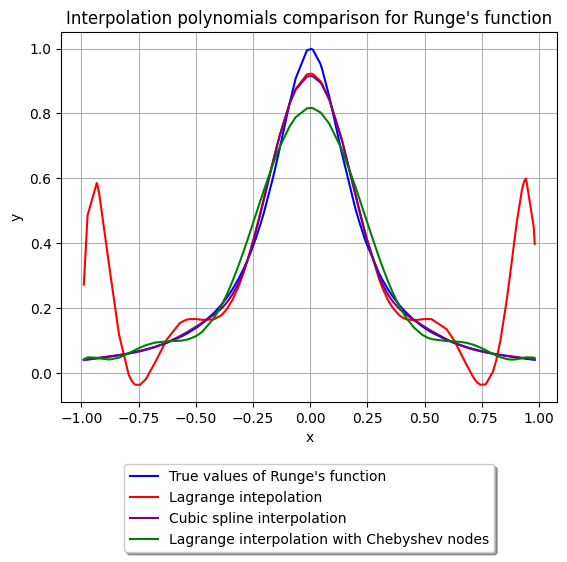
\includegraphics[width=\linewidth]{figures/interpolation.png}
\end{figure}



\subsection*{Wnioski}
\null\quad ...

\section*{Źródła}
\begin{itemize}
    \item \url{https://heath.cs.illinois.edu/scicomp/notes/cs450_chapt07.pdf}
\end{itemize}


\end{document}